%Autor: Simon Walker
%Version: 1.0
%Datum: 29.11.2019
%Lizenz: CC BY-NC-SA

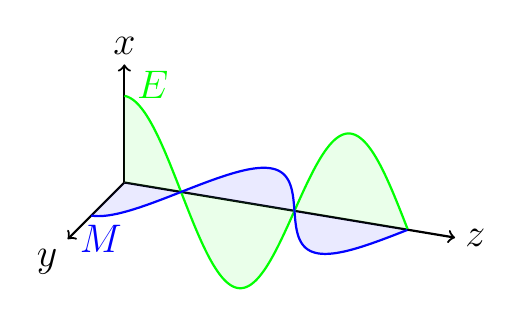
\begin{tikzpicture}[x={(0,1cm)}, y={(-0.6cm,-0.6cm)}, z={(1.2cm, -0.2cm)}]
		
	\def\cycles{1.25} %Anz Schwingungen
	\def\lenght{3}%länge in z richtung
	
	
	\draw [->, thick] (0,0,0)  -- (1.5,0,0) node[above] {\Large$x$};
	\draw [->, thick] (0,0,0) -- (0,1.2,0) node[below left] {\Large$y$};
	\draw [->, thick] (0,0,0) -- (0,0,\lenght+0.5) node[right] {\Large$z$};
	
	\draw[thick, green] %E-Feld Plot
	plot[domain=0:\lenght, samples=200] 
	({1.1*cos(deg(2*\cycles*pi*\x/\lenght))}, 0, \x);
	
	\draw[thick, blue] %M-Feld Plot
	plot[domain=0:\lenght, samples=200] 
	(0, {0.7*cos(deg(2*\cycles*pi*\x/\lenght))}, \x);
	
	\fill[opacity=.1,green!80] %E-Feld füllung
	(0,0,0) --
	plot[domain=0:\lenght, samples=200] 
	({1.1*cos(deg(2*\cycles*pi*\x/\lenght))}, 0, \x)  --
	(0,0,0);
	
	\fill[opacity=.1,blue!80] %M-Feld füllung
	(0,0,0) --
	plot[domain=0:\lenght, samples=200] 
	(0, {0.7*cos(deg(2*\cycles*pi*\x/\lenght))}, \x)  --
	(0,0,0);
	
	\node[green] at (1.3,0,0.3) {\Large$E$}; %Beschriftungen
	\node[blue] at (0,1.1,0.3) {\Large$M$};
	
\end{tikzpicture}
